\documentclass{RVTM}

\usepackage{lipsum}
\usepackage{wrapfig}


\title{This is the title of this document}


\begin{document}

\rvtmtoc


\setcounter{page}{18}
\chapter{Introduction}

\rvtmepigraph{Some long citation}[Some author]

\section{Section}


\lipsum[1]
 
\section{Section} 
 
\subsection{Subsection}


\lipsum[2]

\hdottedline%
\begin{multicols}{2}
	\lipsum[3]
\end{multicols}
  


\subsection{Subsection}

\lipsum[4]



\ycard[inversed][padding=2em]{%
	\yccontent{%
		\framedpagetitle{Test}
		\lipsum[2]}
}
\lipsum[1]


\begin{framedpage}
	{\centering%
		\framedpagetitle{Test}
	}
	\lipsum[1]
\end{framedpage}

\begin{blackpage}
	\framedpagetitle{Test}
	\lipsum[1]
\end{blackpage}

\begin{bpdp}{images/Icelandic_Roads_Faded_26.jpg}%
	\noindent%
	\begingroup
	\color{white}%
	\sffamily\bfseries%
	\vfill
	\begin{center}
		\fontsize{2cm}{2.4cm}\selectfont\highcontrastfont%
		ICELAND\\[1cm]
		\rule{.5\linewidth}{5mm}
	\end{center}
	
	\vfill%
	\noindent\lipsum[3]
	\vfill
	\vfill
	\endgroup
	
	\bpdpnewpage%
	\null%
	\vfill
	\hspace*{-1em}\ycard[][padding = 1.5cm, content/align=justify]{
		\yccontent{
			\framedpagetitle{\highcontrastfont Test}
			\begin{wrapfigure}{l}{.6\linewidth}
				\vspace*{-\baselineskip}
				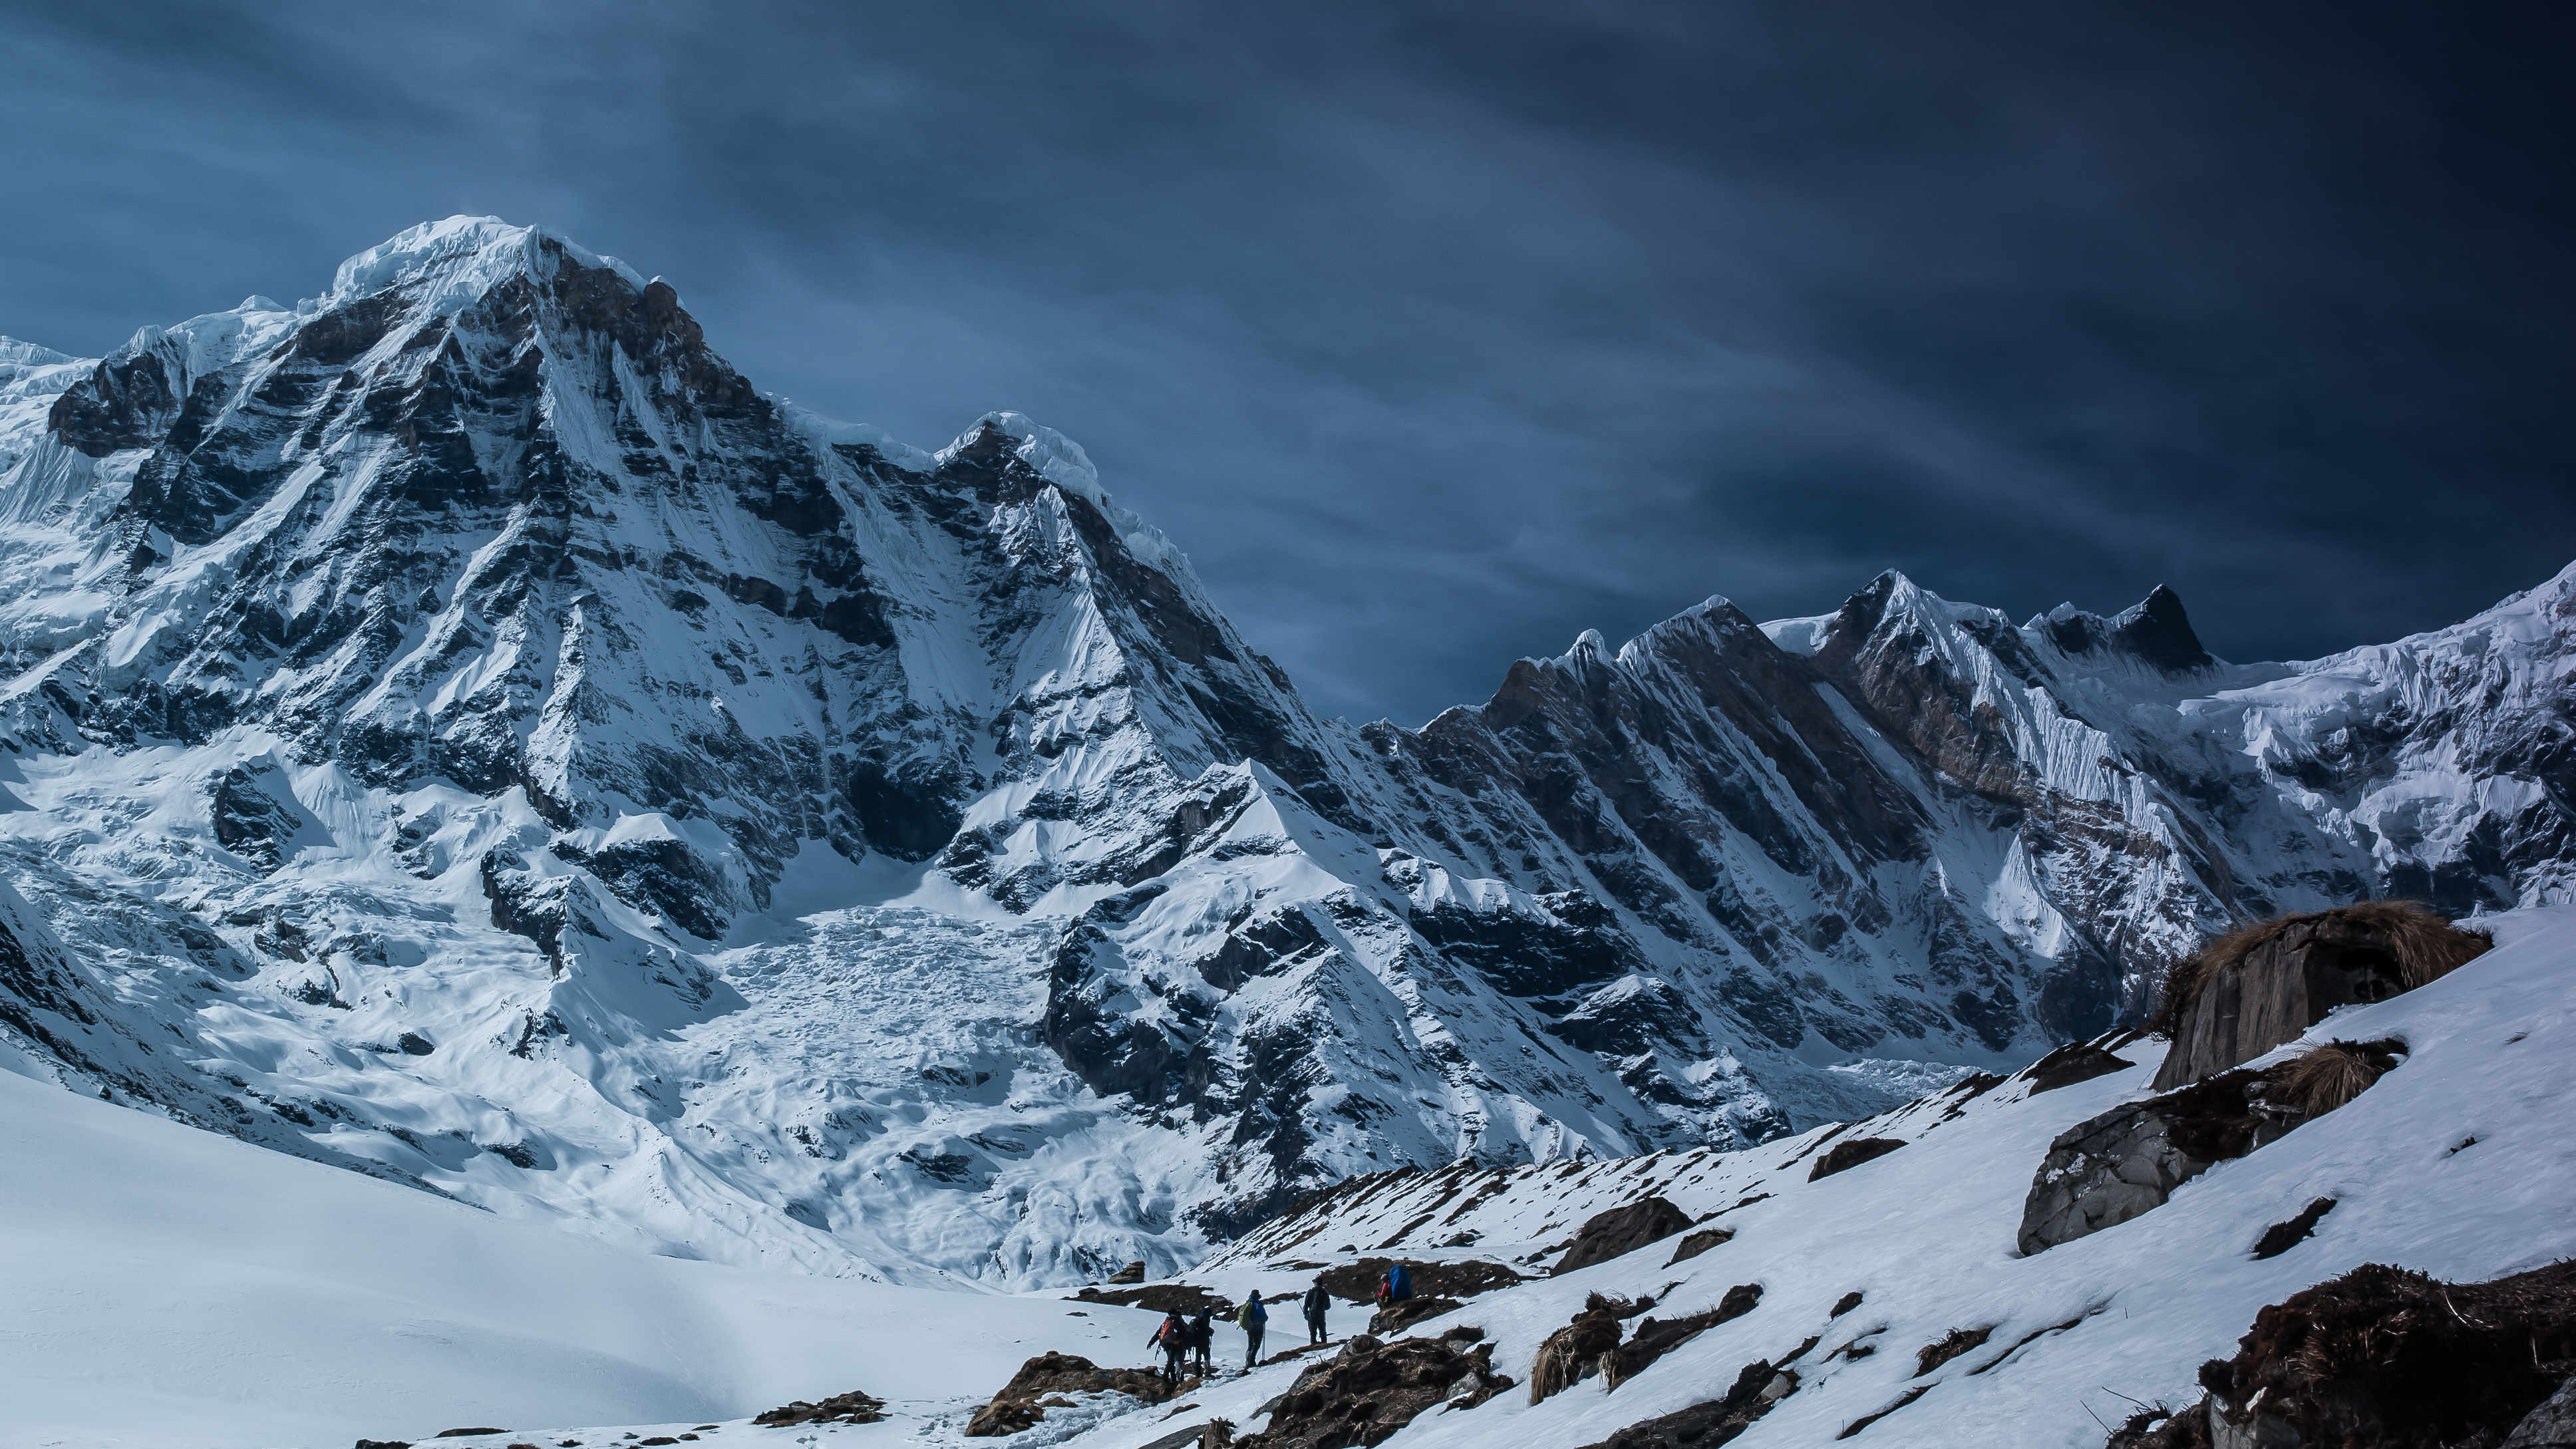
\includegraphics[width=\linewidth]{images/cold-snow-winter-mountain.jpeg}
			\end{wrapfigure}
			\lipsum[1]
			\vspace{2\baselineskip}
			\begin{wrapfigure}{r}{.6\linewidth}
				\vspace*{-\baselineskip}
				\includegraphics[width=\linewidth]{images/pexels-photo-213703.jpeg}
			\end{wrapfigure}
			\lipsum[1]
		}
	}
	\vfill%
\end{bpdp}

\begin{quotationpage}[Mary Wollstonecraft]
	Il semble que les hommes, en général, préfèrent utiliser leur raisonnement, à justifier les préjugés qu’ ils ont assimilés sans trop savoir comment plutôt qu'à les déraciner.
\end{quotationpage}

\begin{quotationpage}[Mary Wollstonecraft][black quotation page]%
	Il semble que les hommes, en général, préfèrent utiliser leur raisonnement, à justifier les préjugés qu’ ils ont assimilés sans trop savoir comment plutôt qu'à les déraciner.
\end{quotationpage}

\setcounter{page}{30}
\chapter{A Chapter}
%
%
\setcounter{page}{36}
\chapter{A Further Chapter}

\setcounter{page}{46}
\chapter{An even further chapter}

\setcounter{page}{54}
\chapter{Well... You get the idea}
%
\setcounter{page}{62}
\chapter{Now I am running out of idea}

\setcounter{page}{89}
\chapter{But hopefully I am soon at the end}

\setcounter{page}{102}
\chapter{The End}

\end{document}
